\chapter{TDD pattern of the OFDM frame}
\label{chap:TDD pattern of the OFDM frame}


Initially, sensing radar processing was performed on a per OFDM frame basis. \protect\newline Every $10$ ms the system would output a received OFDM frame for radar processing, generating a target state update. When the entire frame is processed, the number of subcarriers and symbols is quite large, resulting in good radar performance and significant SNR gain after computing the periodogram. However, this approach suffers from the presence of unwanted spectral replicas caused by the presence of empty uplink (UL) symbols in the frame.
    
As shown in section \ref{sec:intro-PoCarchitecture}, the gNB transmits in a TDD pattern. Each pattern consists of 104 DL symbols and 36 UL symbols, repeated 8 times in each frame.

Received UL symbols do not contain any useful information for radar processing, hence they are discarded (set to zero) before computing the periodogram.

\begin{figure}[H]
    \centering
    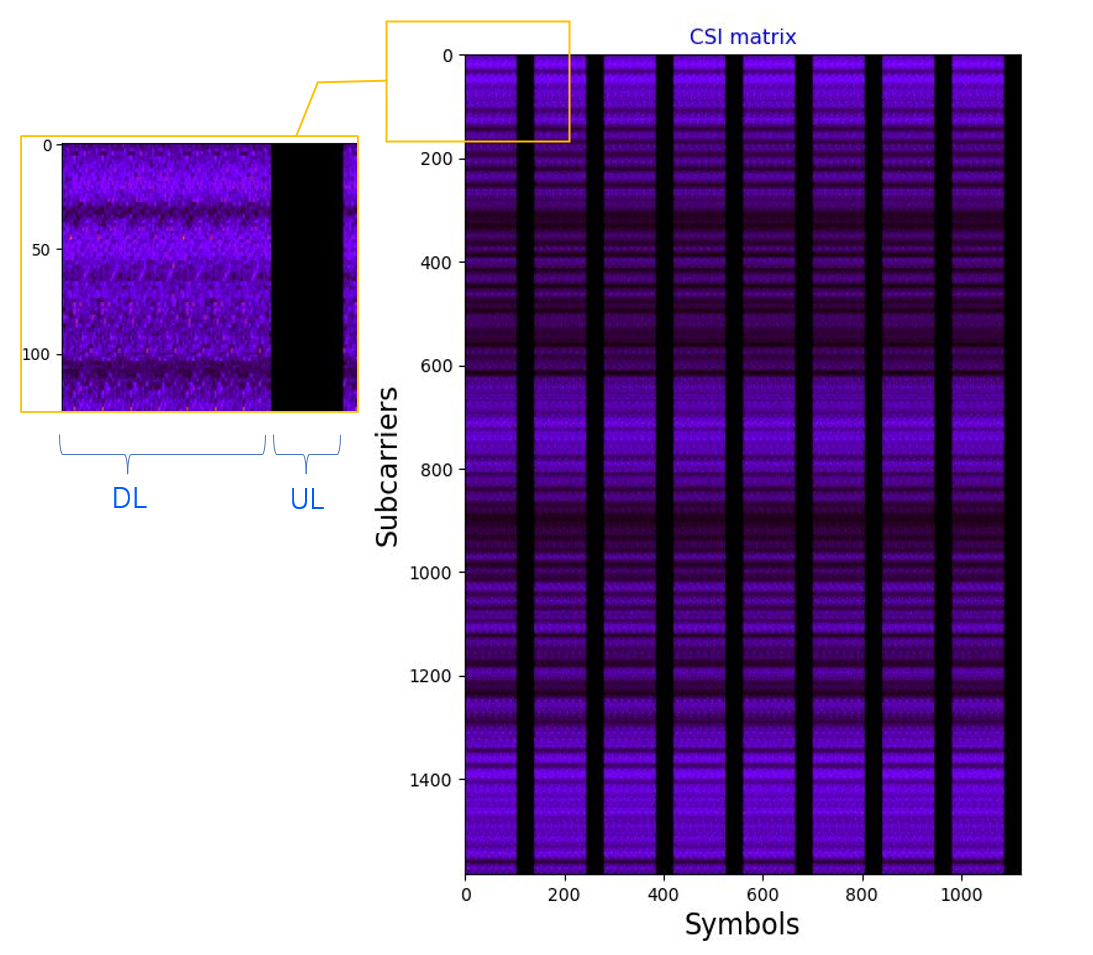
\includegraphics[width=0.5\textwidth]{Images/TDDprocessing/CSIMatrix_DLULpattern.png}
    \caption{CSI matrix from NOKIA PoC, rows and columns correspond to OFDM subcarriers and symbols respectively}
    \label{fig:CSIMatrix_DLULpattern}
\end{figure}

\section{Ideal system performance}

Without modifying the OFDM frame, the system can carry out radar processing with the following performance:

\begin{itemize}
    \item \textbf{Unambiguous speed}
     \vspace{-\baselineskip} % Remove extra whitespace
            \begin{equation}
                v_{\text{unamb}} = \frac{c_0}{2f_C T_S} = 613,15\text{ m/s}.
            \end{equation}
           
     \item \textbf{Unambiguous range}
            \begin{equation}
                d_{\text{unamb}} = \frac{c_0}{2\Delta_f} = 1250,0\text{ m}.
            \end{equation}
     \item \textbf{Speed resolution}
            \begin{equation}
                v_{\text{res}} = \frac{c_0}{2T_Sf_CM} = 0,603 \text{ m/s}.
            \end{equation} 
     \item \textbf{Range resolution}
            \begin{equation}
                d_{\text{res}} = \frac{c_0}{2\Delta_fN} = 0,789 \text{ m}.
            \end{equation}  
\end{itemize}



\section{Effect of empty UL symbols}
    
    The removal of UL symbols acts as windowing on the received frame. This introduces additional spectral replicas in speed as shown in figure \ref{fig:SpectralReplicasDLULpattern}. Replicas seem to appear at a constant speed displacement from where actual targets lie, behaving similarly to replicas due to the radar's non-ambiguity speed.
    
    \begin{figure}[H]
        \centering
        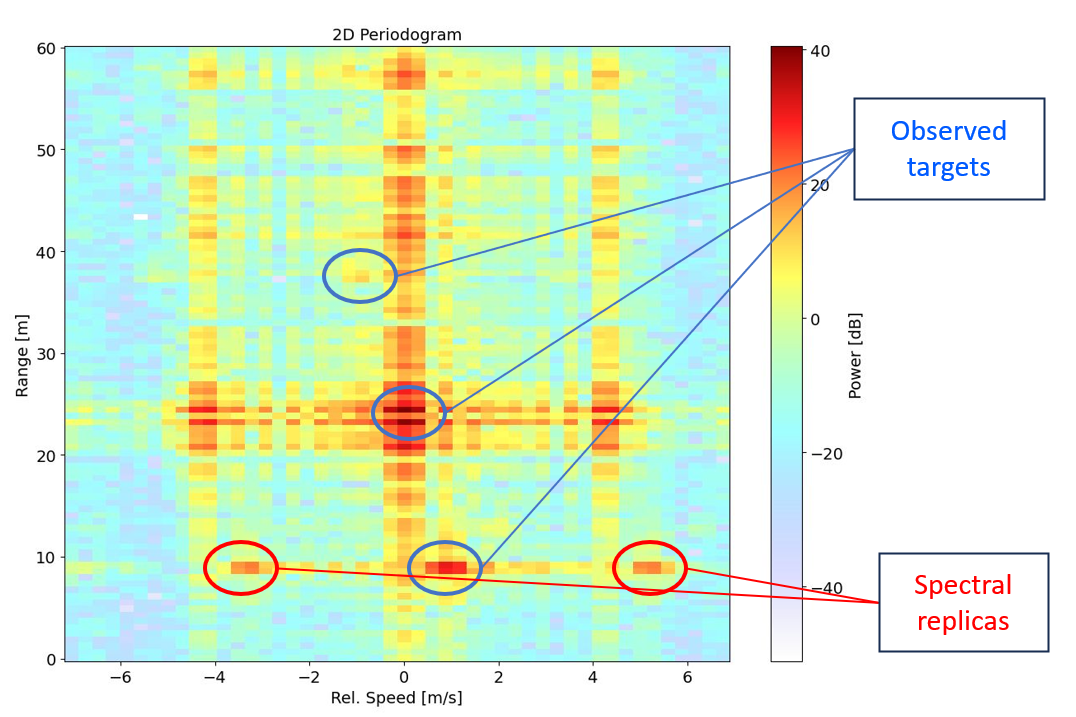
\includegraphics[width=0.55\textwidth]{Images/TDDprocessing/SpectralReplicasDLULpattern.png}
        \caption{Periodogram of a radar measurement with: static target at 23 m; moving target (range = 9,5 m, speed = 0,94 m/s); NLOS target (range = 37,2 m, speed = -1 m/s)}
        \label{fig:SpectralReplicasDLULpattern}
    \end{figure}
    
    In order to characterize the additional spectral replicas, the windowing function used to set all UL symbols to zero is analyzed. The windowing pattern can be expressed in the form
    
    \begin{align}
        &\text{rect}\left( \frac{t + \tau}{104 \cdot T_S}\right) \ast \sum_{i=0}^7 \delta\left( t - i\cdot \frac{140}{1120}\cdot T_{\text{frame}} \right),  \\
        &T_{\text{frame}} = 1120 \cdot T_S.
    \end{align}

    The windowing function, apart from a time-shift factor, is a rectangle function (Dirichlet window) convoluted with a train of Dirac deltas with spacing of 140 samples, Figure \ref{fig:TDDproc_rectfunct}. Its transform in frequency, Figure \ref{fig:TDDproc_rectfunct_transform}, is a cardinal sine function multiplied by a train of Dirac deltas.

    The transform is then convoluted with the signal in the frequency domain. The impulses adjacent to the one at zero-frequency in figure \ref{fig:TDDproc_rectfunct_transform} appear as replicas in the periodogram. These peaks have enough power to be detected as actual targets, limiting the system's performance by reducing the effective unambiguous speed or by masking actual targets that would be detected near the replica. 

\begin{figure}[H]
    \centering
    
    \subfloat[TDD windowing function.\label{fig:TDDproc_rectfunct}]{%
        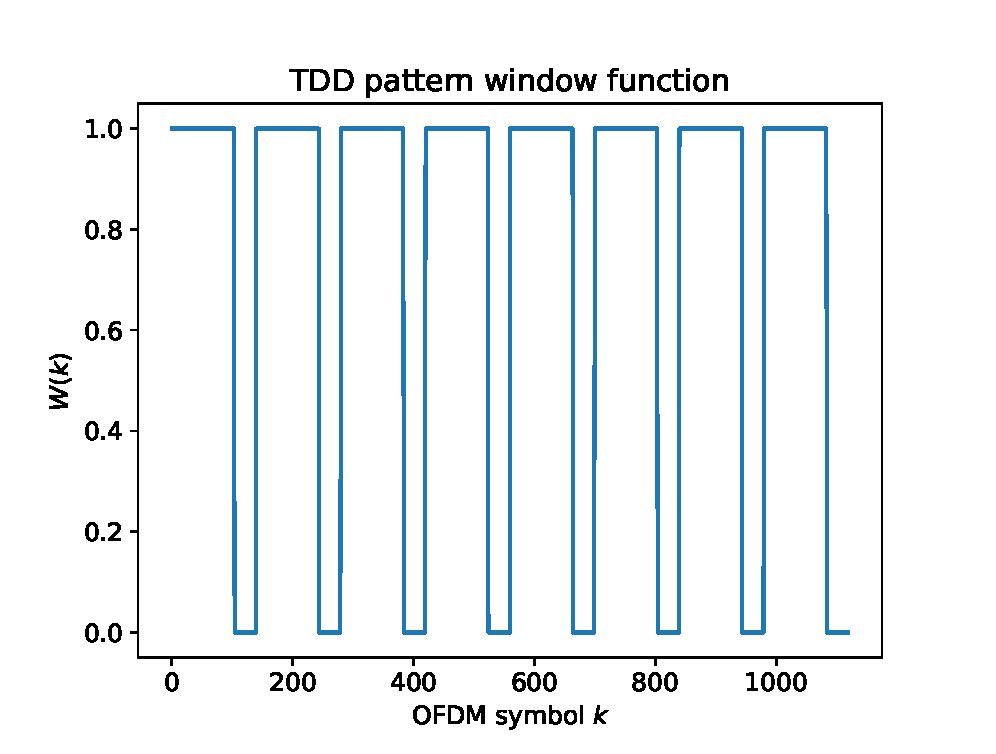
\includegraphics[scale=0.49]{Images/TDDprocessing/TDD_win.eps}%
    }\hfill
    \subfloat[Periodogram of the windowing function, FFT over 2048 points.\label{fig:TDDproc_rectfunct_transform}]{%
        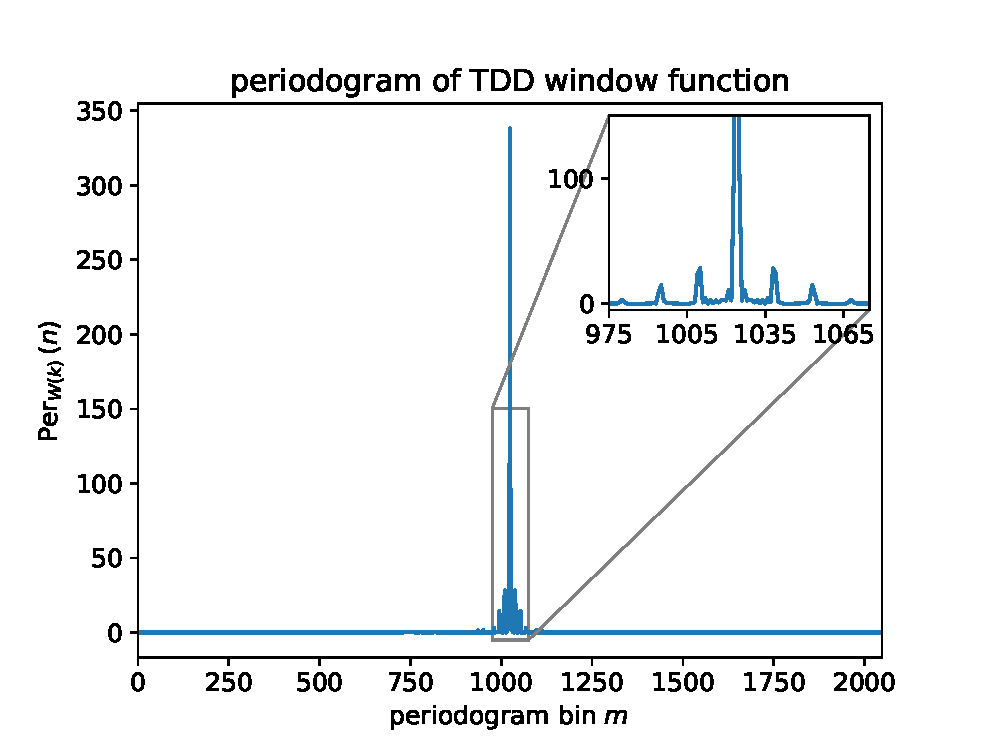
\includegraphics[scale=0.49]{Images/TDDprocessing/periodogram_of_TDD_win.eps}%
    }
    
    \caption[]{}
    \label{fig:TDDwindowingfunct}
\end{figure}

\section{Frame sampling strategies}

    \begin{figure}[H]
        \centering
        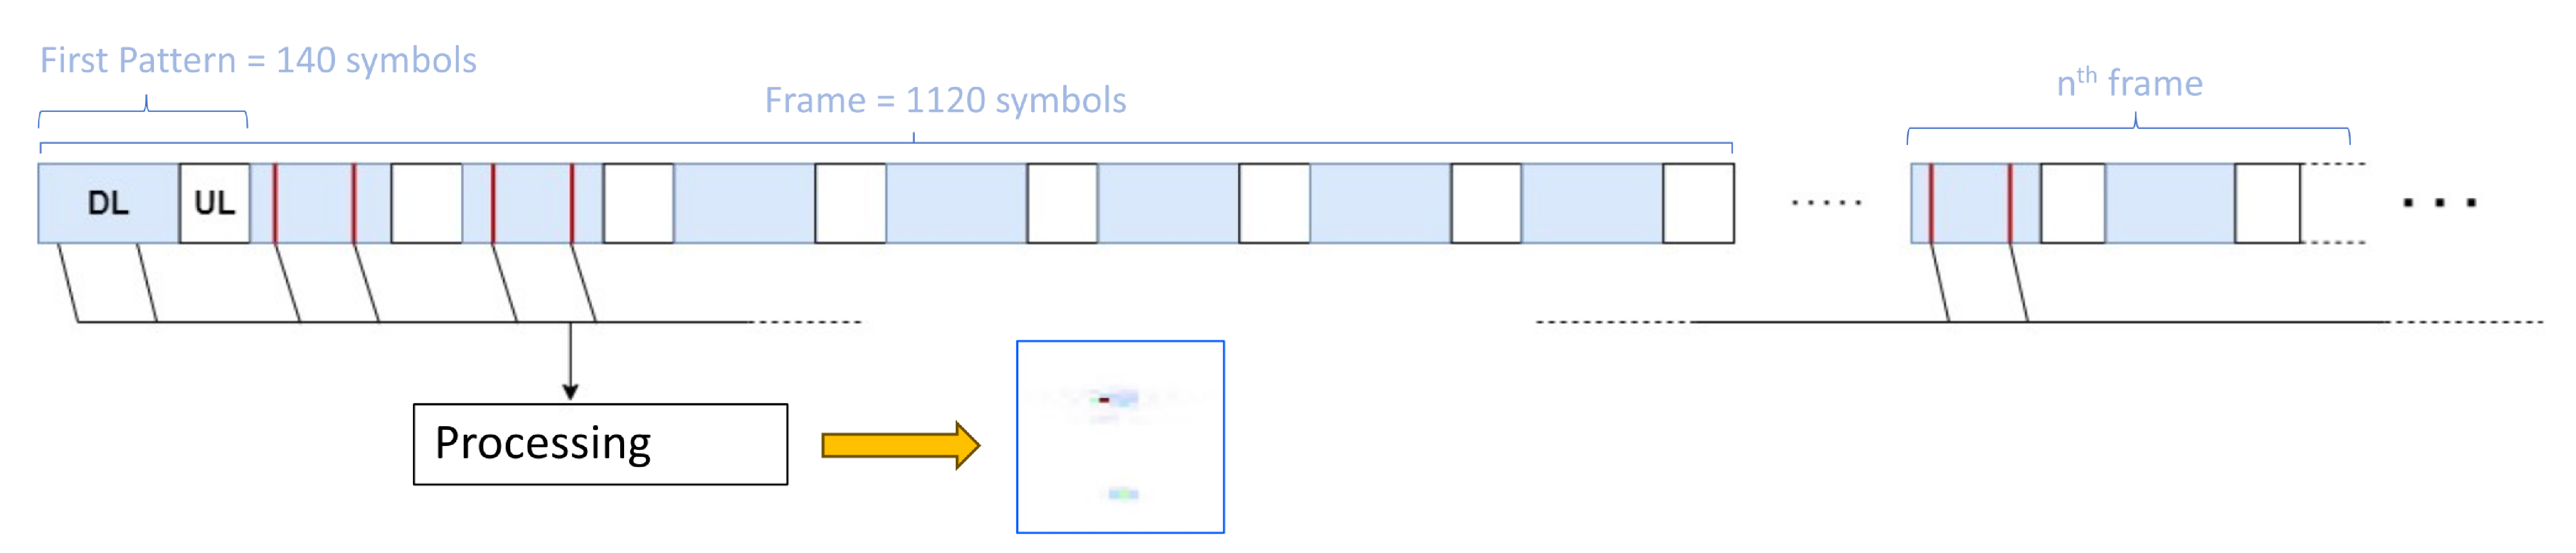
\includegraphics[width=1\textwidth]{Images/TDDprocessing/TDDstrategies.eps}
        \caption{Decimation and combining of different consecutive frames}
        \label{fig:TDDstrategies}
    \end{figure}

    \paragraph{Single DL pattern:}
    in order to avoid processing blank UL symbols, the most straightforward approach would be processing only the first 104 DL symbols. The replicas would be avoided, but the time aperture of the measure would be reduced by a factor 8, decreasing the speed resolution from $0,603$ m/s to $\approx 5,88$ m/s, unusable for most of the sensing use cases.
    
    \paragraph{Decimation at constant interval:}
     a possible strategy is re-sampling the OFDM frame in time at a fixed pace, avoiding blank symbols. Replicas are not detected, but the lower number of processed symbols translates into a considerable loss of SNR in the periodogram. This affects NLOS sensing in particular, since targets observed from a reflection present a considerably lower peak power compared with the LOS components.

     Reducing the number of available symbols with a fixed time-aperture translates in lower granularity of measurements and in a decrease in unambiguous speed. \protect\newline In the case of Figure \ref{fig:TDDperiodogram1FYesDec}, processing one symbol every 47, the obtained unambiguous speed is $13,05$ m/s. \protect\newline Speed resolution remains unchanged.
    
     \paragraph{Decimation and multi-frame processing:}
     combining consecutive frames, it is possible to process an higher number of symbols, re-gaining a part of the SNR thanks to processing gain, all without observing replicas. The time aperture of the measurement is also increased, translating into a better speed resolution.

     This approach introduces a trade-off between SNR (processing gain) and update rate. Increasing the time-aperture, some range migration effect can be observed, especially for fast moving targets. In the context of NLOS sensing, the impact of range migration on system performance is relatively minor compared to the benefits of increased speed resolution and higher signal-to-noise ratio, since the primary goal is not providing precise tracking or positioning data.


% 2x2 figure scheme
    \begin{figure}[H]
        \centering
        
        \subfloat[Single processed frame, no decimation, SNR = 60,91 dB, \protect\newline $v_{\text{res}} = 0,603$ m/s, $ v_{\text{unamb}} = 613,15$ m/s
\label{fig:TDDperiodogram1FNoDec}]{
            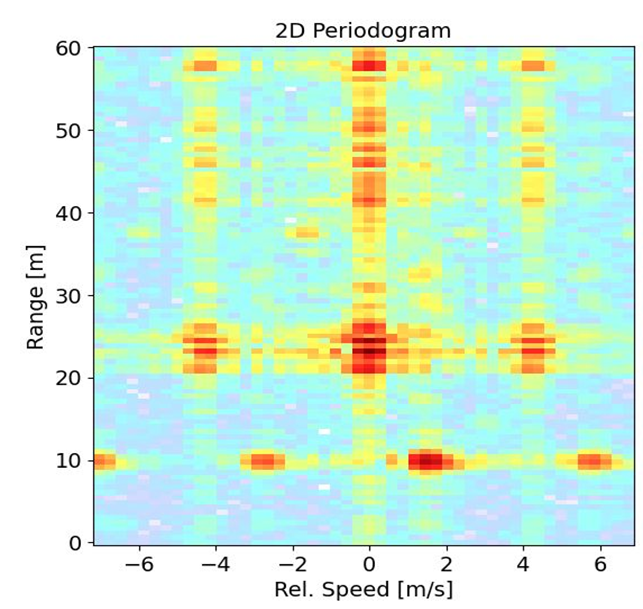
\includegraphics[width=0.4\textwidth]{Images/TDDprocessing/periodogram1FNoDec.png}
        }
        \hfill
        \subfloat[Single processed frame, decimated, \protect\newline SNR = 45,16 dB, \protect\newline $v_{\text{res}} = 0,603$ m/s, $ v_{\text{unamb}} = 13,05$ m/s\label{fig:TDDperiodogram1FYesDec}]{
            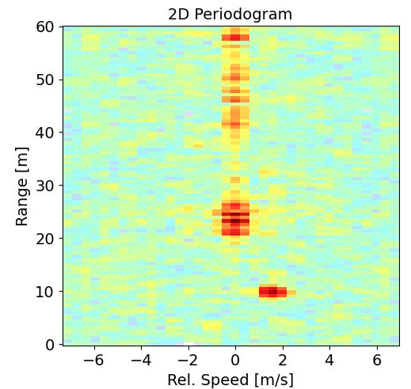
\includegraphics[width=0.4\textwidth]{Images/TDDprocessing/periodogram1FYesDec.png}
        }
        
        \vspace{0.5cm}
        
        \subfloat[6 processed frames, decimated, combined, SNR = 52,35 dB, \protect\newline $v_{\text{res}} = 0,091$ m/s, $ v_{\text{unamb}} = 8,76$ m/s\label{fig:TDDperiodogram6frames}]{
            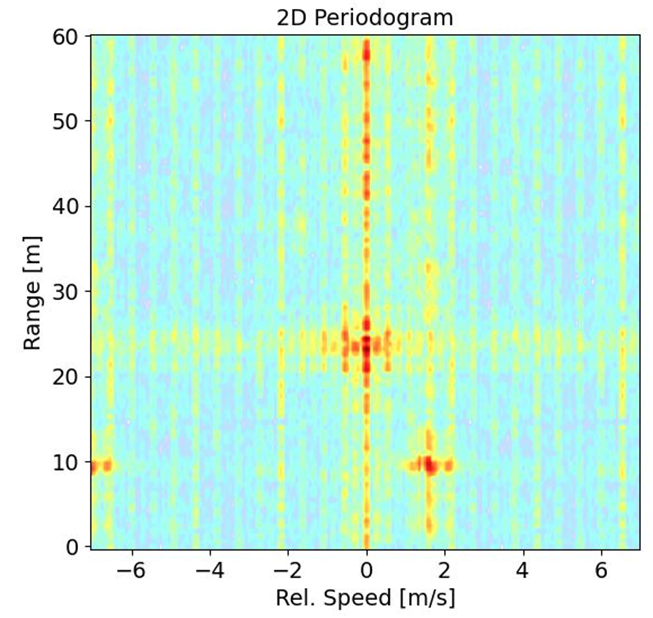
\includegraphics[width=0.4\textwidth]{Images/TDDprocessing/periodogram6frames.png}
        }
        \hfill
        \subfloat[10 processed frames, decimated, combined, SNR = 54.66 dB, \protect\newline $v_{\text{res}} = 0,054$ m/s, $ v_{\text{unamb}} = 8,76$ m/s\label{fig:TDDperiodogram10frames}]{
            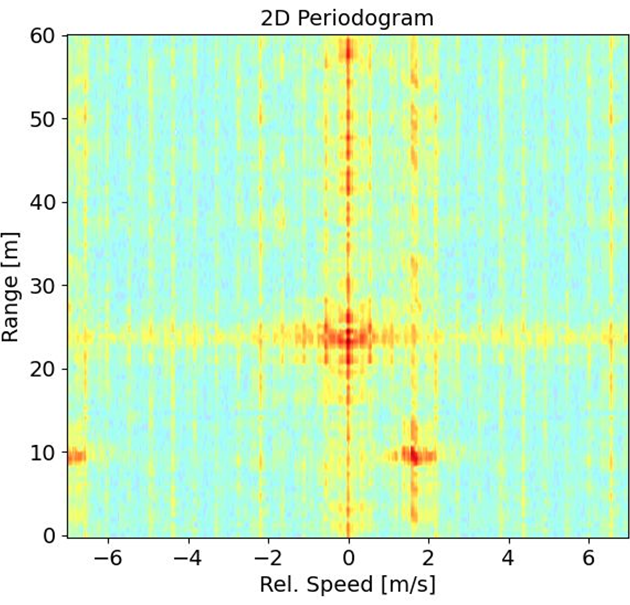
\includegraphics[width=0.4\textwidth]{Images/TDDprocessing/periodogram10frames.png}
        }
        
        \caption{Examples of possible decimation and combining approaches in periodogram processing}
        \label{fig:allperiodogram-decimation}
    \end{figure}

    In Figures \ref{fig:TDDperiodogram1FNoDec}-\ref{fig:TDDperiodogram10frames} it is possible to observe the effects of the various strategies when applied to a OFDM radar measurement where both the NLOS and LOS components are present for a single target.

	In order to increase the number of available frames, the processed frame stride can be set to be lower then the number of combined frames. Letting the processed time-window overlap allows to increase the target update rate of the system.

    
\begin{table}[H]
    %\caption*{\textbf{Title of Table (optional)}}
    \centering 
    \begin{tabular}{|p{9em} c c c |}
    \hline
    \rowcolor{bluepoli!40} % comment this line to remove the color
     \textbf{Strategy} & \textbf{SNR [dB]} & \textbf{N} & \textbf{Time aperture [ms]} \T\B \\
    \hline \hline
    $\textbf{Standard frame}$ & 60,91 & 1120 & 10 \T\B \\
    $\textbf{Decimated frame}$ & 45,16 & 24 & 10 \T\B\\
    $\textbf{6 frames}$ & 52,35 & 96 & 60  \T\B\\
    $\textbf{10 frames}$ & 54,66 & 160 & 100  \T\B\\

    \hline
    \end{tabular}
    \\[10pt]
    \caption{Comparison between SNR levels for different frame processing strategies}
    \label{table:TDDstratcomparison}
\end{table}


\section{Effect of CP removal in multiple frame processing}
